\documentclass[12pt,xcolor=table,aspectratio=169]{beamer}
\usetheme{Frankfurt}
\usecolortheme{rose}
\usepackage{amsthm}
\usepackage{amsmath}
\usepackage{bbm}
\usepackage{amsfonts}
\usepackage{amssymb}
\usepackage{graphicx}
\usepackage{hyperref}
\usepackage[flushleft]{threeparttable}
\usepackage{tabularx}
\usepackage{booktabs}
\usepackage{siunitx}
\usepackage{tikz}
\usetikzlibrary{decorations.pathreplacing,angles,quotes}
%\usepackage{enumitem}% http://ctan.org/pkg/enumitem

%set up course and number

\newcommand{\ClassName}{TBD}
\newcommand{\ClassNumber}{TBD}
\newcommand{\Topic}{TBD}

% Some optional colors. Change or add as you see fit.
%---------------------------------------------------
 \definecolor{ualbertagreen}{HTML}{007C41}
\definecolor{ualbertagold}{HTML}{FFDB05}

\definecolor{calloutgrey}{HTML}{D9D9D9}


%set fonts
\setbeamerfont{subtitle}{size=\large,shape=\scshape,series=\bfseries}
\setbeamerfont{title}{size=\Large,shape=\scshape,series=\bfseries}
\setbeamerfont{author}{size=\large}
\setbeamerfont{date}{size=\large}
\setbeamerfont{caption}{size=\scriptsize}


% Some optional color adjustments to Beamer. Change as you see fit.
%------------------------------------------------------------------
\setbeamercolor{frametitle}{fg=ualbertagreen,bg=white}
\setbeamercolor{title}{fg=ualbertagreen,bg=white}
\setbeamercolor{author}{fg=ualbertagreen,bg=white}
\setbeamercolor{date}{fg=ualbertagreen,bg=white}
\setbeamercolor{local structure}{fg=ualbertagreen}
\setbeamercolor{section in toc}{fg=ualbertagreen,bg=white}
% \setbeamercolor{subsection in toc}{fg=ualbertagreen,bg=white}
\setbeamercolor{footline}{fg=ualbertagreen!50, bg=white}

% definition boxes
\setbeamercolor{block title}{bg=ualbertagreen,fg=white}
\setbeamercolor{block body}{parent=normal text,use=block title,bg=calloutgrey}
%\setbeamercolor{block body}{parent=normal text,use=block title,bg=block title.bg!30!bg}


\setbeamercolor{upper separation line head}{bg=ualbertagreen}
\setbeamercolor{lower separation line head}{bg=ualbertagold}
\setbeamercolor{middle separation line head}{bg=ualbertagold}
\setbeamercolor{frametitle}{fg=ualbertagreen,bg=white}



\setbeamercolor{section in head/foot}{bg=white,fg=ualbertagreen}
\setbeamercolor{author in head/foot}{bg=white,fg=ualbertagreen}
\setbeamercolor{date in head/foot}{bg=white,,fg=ualbertagreen}
\setbeamercolor{title in head/foot}{bg=white,fg=ualbertagreen}

\setbeamercolor{headline}{bg=white,fg=ualbertagreen}




\setbeamercolor*{middle separation line head}{bg=ualbertagreen}
\setbeamercolor*{alerted text}{fg=ualbertagreen}
\setbeamercolor*{example text}{fg=black}
\setbeamercolor*{structure}{fg=black}


\let\Tiny=\tiny



\logo{
   %\ifnum\insertpagenumber>1
   \tikz [remember picture,overlay]
    \node[yshift=.3cm,xshift=1.5cm] at (current page.south west)
        %or: (current page.center)
        {
\includegraphics[width=1in]{../images/UA-ASB-COLOUR.png}};
    %\fi
%
\includegraphics[height=0.8cm]{../images/UA-ASB-COLOUR.png}\vspace{220pt}
}


\setbeamertemplate{title page}{%
  \vbox{}
    \vspace{.5cm}% NEW
  \begingroup
    \centering
    \begin{beamercolorbox}[sep=8pt,center]{title}
      \usebeamerfont{title}\ClassNumber: \ClassName\par%
      \usebeamerfont{title}\inserttitle\par%
     \ifx\insertsubtitle\@empty%
      \else%
        \vskip0.05em%
        {\usebeamerfont{subtitle}\usebeamercolor[fg]{subtitle}\insertsubtitle\par}%
      \fi%
    \end{beamercolorbox}%
    \begin{beamercolorbox}[sep=8pt,center]{author}
      \usebeamerfont{author}\insertauthor
    \end{beamercolorbox}
    \begin{beamercolorbox}[sep=8pt,center]{institute}
      \usebeamerfont{institute}\insertinstitute
    \end{beamercolorbox}

    \vspace{0.5cm}% NEW
    \begin{beamercolorbox}[sep=8pt,center]{date}
      \usebeamerfont{date}\insertdate
    \end{beamercolorbox}\vskip0.05em

      \endgroup
  %\vfill
}


\setbeamertemplate{frametitle}{%
    \insertframetitle\par\vskip-10pt
}



\renewcommand{\ClassName}{Business Economics, Organization and Management}
\renewcommand{\ClassNumber}{BUEC 311}

\setbeamertemplate{headline}{%
\leavevmode%
 \hbox{%
    \begin{beamercolorbox}[wd=\paperwidth,ht=5ex,dp=0ex]{white}%
    \usebeamerfont{headline}\hskip6pt\ClassNumber: \inserttitle\par%
    \insertsectionnavigationhorizontal{\paperwidth}{}{\hskip0pt plus1filll}
    \end{beamercolorbox}%
  }
}

\defbeamertemplate*{footline}{my footline}{%
    \ifnum\insertpagenumber=1
        \Tiny{%
            \hfill%
		\vspace*{1pt}%
            %\insertframenumber/\inserttotalframenumber \hspace*{0.1cm}%
            \newline%
            \color{ualbertagold}{\rule{\paperwidth}{0.4mm}}\newline%
            \color{ualbertagold}{\rule{\paperwidth}{.4mm}}%
        }
  \else%
        \Tiny{%
            \hspace{.66\paperwidth}
            %\vspace{25pt}
            \insertframenumber/\inserttotalframenumber
            \newline%
            \color{ualbertagold}{\rule{\paperwidth}{0.4mm}}\newline%
            \color{ualbertagold}{\rule{\paperwidth}{.4mm}}%
        }%
    \fi%
}


\newenvironment{itemize*}%
  {\begin{itemize}%
    \setlength{\itemsep}{0pt}%
    \setlength{\parskip}{0pt}}%
  {\end{itemize}}


\title{Strategic Behaviour Part I\\
	Game Theory and Business Strategy
}

\date{Fall 2020}

\begin{document}

\section{Overview}


\frame{
	\titlepage
}

\frame{
	\frametitle{Outline}
	\begin{enumerate}
	\item Oligopoly Games
	\item[]
	\item Nash Equilibrium
	\item[]
	\item Information and Rationality
	\item[]
	\item Using Game Theory to Make Business Decisions
	\item[]
	\item Bargaining
	\item[]
	\item Auctions
	\end{enumerate}
}

\frame{
	\frametitle{Strategic Interaction}
	\begin{itemize}
	\item Thus far: We have primarily focused on cases where firms are not interacting strategically.
		\begin{itemize}
		\item But we often need to understand the potential decisions of rivals.
		\item We need a toolbox for understanding strategic decision making.
		\end{itemize}
	\item[]
	\item \underline{Game Theory}: A set of tools used to analyze strategic decision making.
		\begin{itemize}
		\item Idea: Model strategic interactions as a \underline{game} in which \underline{players} interact according to a set of rules.
			\begin{itemize}
			\item Players decide \underline{strategies} based on \underline{payoffs}, the level of \underline{information}, and their \underline{rationality}.
			\item Outcome of a game is a \underline{Nash Equilibrium}; depends on information and rationality.
			\end{itemize}
		\item Game theory can be used to understand strategic behaviour by firms, outcomes in bargaining, and auctions.
		\end{itemize}
	\end{itemize}
}

\frame{
	\frametitle{Outline}
	\begin{enumerate}
	\item \alert{Oligopoly Games}
	\item[]
	\item Nash Equilibrium
	\item[]
	\item \strikethrough{Information and Rationality}
	\item[]
	\item Using Game Theory to Make Business Decisions
	\item[]
	\item Bargaining
	\item[]
	\item Auctions
	\end{enumerate}
}

\section{Oligopoly Games}


\frame{
	\frametitle{Oligopoly Games}
	\begin{itemize}
	\item Ex. A duopoly game between American Airlines and United Airlines
		\begin{itemize}
		\item Players and rules:
			\begin{itemize}
			\item \underline{Two players}: American and United, play a \underline{static game} to decide how many passengers to fly per quarter. Each airline's objective is to maximize profit.
			\item \underline{Rules}: Firms announce output levels \underline{simultaneously}, but cannot communicate otherwise (no side deals or coordination is allowed).
			\item \underline{Complete information}: Firms know all strategies and payoffs.
			\end{itemize}
		\item[]
		\item Strategies:
			\begin{itemize}
			\item Each firm's \underline{strategy} is to take one of two available actions: ether choose low output (48k passengers per quarter) or high output (64k passengers per quarter).
			\item Both firms know all strategies and the corresponding payoffs for each firm.
			\item We can summarize these strategies in a payoff matrix (or profit matrix).
			\end{itemize}
		\end{itemize}
	\end{itemize}
}

\frame{
	\frametitle{Oligopoly Games}
	\begin{figure}
	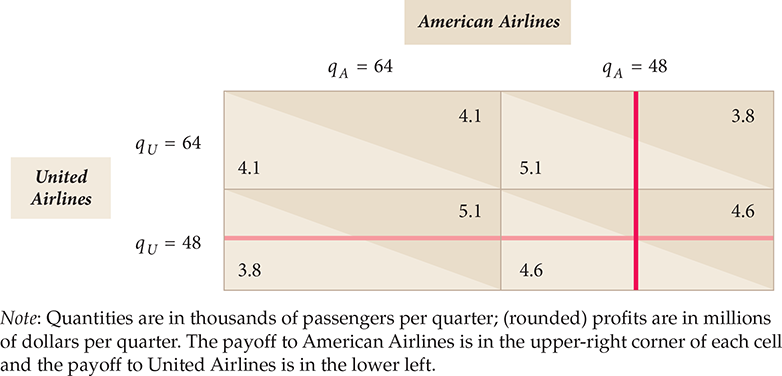
\includegraphics[scale=0.4]{../images/game_theory/au1.png}
	\caption{The Payoffs for American and United}
	\end{figure}
}

\frame{
	\frametitle{Dominant Strategies}
	\begin{itemize}
	\item If one is available, a rational player always uses a \underline{dominant strategy}.
	\end{itemize}
	\begin{definition}[Dominant Strategy]
	A dominant strategy is a strategy that produces a higher payoff (profit) than any other strategy the player can use, no matter what its rivals do.
	\end{definition}
	\begin{itemize}
	\item In our airline duopoly example, high-output (64k) is the dominant strategy for both firms.	
		\begin{itemize}
		\item High output yields the highest profit \textit{regardless of what the other firm is doing}.
		\item Hence, the \underline{dominant strategy solution} is $q_{U} = q_{A} =64$.
		\end{itemize}
	\end{itemize}
}

\frame{
	\frametitle{Payoffs}
	\begin{itemize}
	\item A dominant strategy solution does not necessarily lead to the best outcome for firms.
		\begin{itemize}
		\item In our example, United and American choose strategies that do not maximize their joint or combined profit.
			\begin{itemize}
			\item Each firm could earn \$4.6 million if they both chose to produce a low level of output (48k).
			\end{itemize}
		\item[]
		\item Game between United and American is an example of a \underline{Prisoner's Dilemma}.
			\begin{itemize}
			\item All players have dominant strategies that lead to a profit that is inferior to what they could have achieved if they cooperated.
			\item Individual incentives cause players to choose strategies that do not maximize joint profits.
			\end{itemize}
		\end{itemize}
	\end{itemize}
}

\frame{
	\frametitle{Prisoner's Dilemma Example}
	\begin{itemize}
	\item Suppose that United and American are now choosing whether or not to invest in new planes. Currently, each airline earns a profit of \$25 billion using their old fleet of planes. If American upgrades to new planes and United does not, then American steals some of United's customers and increases its profits to \$35 billion, while United's profits fall to \$10 billion. Similarly, if United upgrades and American does not, United's profits increase to \$35 billion and American's profits fall to \$10 billion. If both airlines upgrade to new planes, then they each will earn \$20 billion. What will each firm do? What will they earn in equilibrium?
	\end{itemize}
}

\frame{
	\frametitle{Best Responses}
	\begin{itemize}
	\item Many games do not have a dominant strategy solution. In this case, we can use the approach of \underline{best response} to determine the outcome of a game.
	\end{itemize}
	\begin{definition}[Best Response]
	A best response is the strategy that maximizes a players payoff (profit) given its beliefs about the strategies of its rivals.
	\end{definition}
	\begin{itemize}
	\item A dominant strategy is a strategy that is a best response to all possible strategies a rival might use.
	\item[]
	\item In the absence of a dominant strategy, each firm can determine its best response to \underline{any possible} strategy chosen by its rivals.
	\end{itemize}
}

\frame{
	\frametitle{Nash Equilibrium}
	\begin{itemize}
	\item Best responses are the basis of a \underline{Nash Equilibrium}.
	\end{itemize}
	\begin{definition}[Nash Equilibrium]
	A Nash equilibrium is a set of strategies such that if, when all other players use these strategies, no player can obtain a higher profit by choosing a different strategy.
	\end{definition}
	\begin{itemize}
	\item In a Nash equilibrium, players are ``best-responding'' to each other.
		\begin{itemize}
		\item This means the Nash equilibrium is self enforcing.
		\end{itemize}
	\item[]
	\item Two steps to find the Nash Equilibrium:
		\begin{enumerate}
		\item Determine each player's best response to any given strategy of the other player.
		\item Check whether pairs of strategies are best responses for both firms; these pairs are Nash equilibria.
		\end{enumerate}
	\end{itemize}
}

\frame{
	\frametitle{Oligopoly Games}
	\begin{itemize}
	\item As an example, consider a more complicated game between American and United.
		\begin{itemize}
		\item Now both firms have 3 possible strategies:
			\begin{enumerate}
			\item High output (96k passengers/quarter).
			\item Medium output (64k passengers/quarter).
			\item Low output (8k passengers/quarter).
			\end{enumerate}
		\item Otherwise, the rules are the same as before:
			\begin{itemize}
			\item Static simultaneous move game.
			\item Perfect information.
			\end{itemize}
		\end{itemize}
	\end{itemize}
}

\frame{
	\frametitle{Oligopoly Games}
	\begin{figure}
	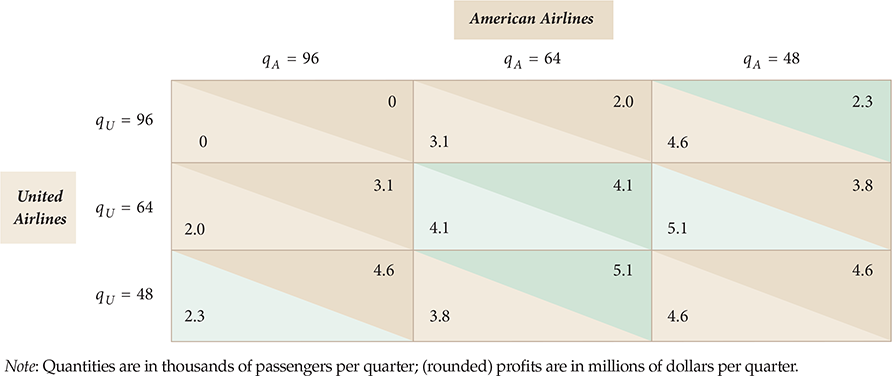
\includegraphics[scale=0.4]{../images/game_theory/au2.png}
	\end{figure}
}

\frame{
	\frametitle{Oligopoly Games}
	\begin{itemize}
	\item Determine equilibrium via two step method:
		\begin{enumerate}
		\item Determine best responses for United:
			\begin{itemize}
			\item If United chooses $q_U=96$, American's best response is $q_{A}=48$.
			\item If United chooses $q_U=64$, American's best response is $q_{A}=64$.
			\item If United chooses $q_U=48$, American's best response is $q_{A}=64$.
			\end{itemize}
		\item[] And for American:
			\begin{itemize}
			\item If American chooses $q_A=96$, United best response is $q_{U}=48$.
			\item If American chooses $q_A=64$, United best response is $q_{U}=64$.
			\item If American chooses $q_A=48$, United best response is $q_{U}=64$.
			\end{itemize}
		\item[]
		\item Determine the Nash Equilibrium
			\begin{itemize}
			\item The Nash equilibrium is $q_{A} = q_{U} = 64$.
			\item This outcome is a Nash equilibrium because neither firm wants to deviate from its strategy \textit{given what the other firm is doing.}
			\item Note: The Nash Equilibrium does not maximize joint profits.
			\end{itemize}
		\end{enumerate}
	\end{itemize}
}

\frame{
	\frametitle{Oligopoly Games}
	\begin{itemize}
	\item In general, whether or not the Nash equilibrium maximizes the combined payoff to players (i.e. profits for firms) depends on the payoff matrix.
	\item[]
	\item As an example, consider a static game where firms decide to `advertise' or `not advertise'.
	\item[]
	\item The effects of advertising depend on whether advertising brings new customers into the market.
	\end{itemize}
}

\frame{
	\frametitle{Oligopoly Games}
	\begin{figure}
	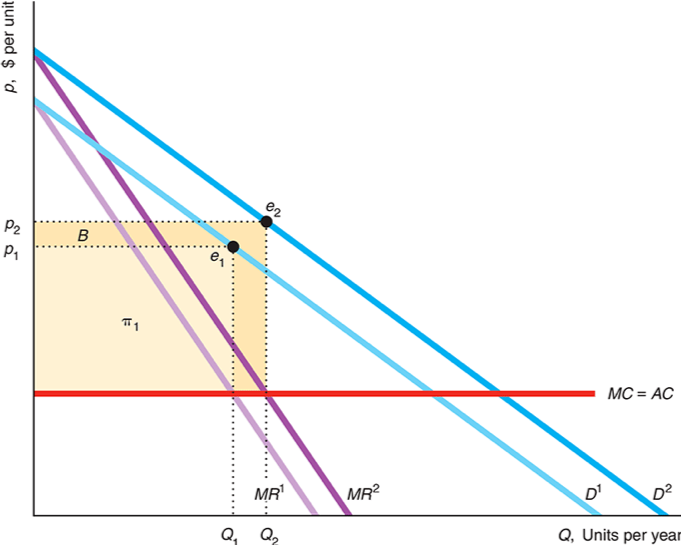
\includegraphics[scale=0.3]{../images/game_theory/advertising.png}
	\end{figure}
}

\frame{
	\frametitle{Oligopoly Games}
	\begin{itemize}
	\item Example highlights a phenomenon often observed in practice:
		\begin{itemize}
		\item In oligopolistic markets, the effect of firm advertising depends on whether it helps (increases the size of the overall market) or hurts (steals customers) rivals.
		\end{itemize}
	\item[]
	\item In some industries, advertising primarily steals customers from rivals.
		\begin{itemize}
		\item E.g. market for cola; market for erectile dysfunction drugs.
		\end{itemize}
	\item[]
	\item In other industries, advertising by any firm increases the size of the market.
		\begin{itemize}
		\item E.g. market for beer; market for cigarettes.
		\end{itemize}
	\item[]
	\item It is possible to observe market size and business stealing effects simultaneously.
		\begin{itemize}
		\item E.g. Fast food; CPUs.
		\end{itemize}
	\end{itemize}
}

\section{Nash Equilibrium}

\frame{
	\frametitle{Outline}
	\begin{enumerate}
	\item Oligopoly Games
	\item[]
	\item \alert{Nash Equilibrium}
	\item[]
	\item Information and Rationality
	\item[]
	\item Using Game Theory to Make Business Decisions
	\item[]
	\item Bargaining
	\item[]
	\item Auctions
	\end{enumerate}
}


\frame{
	\frametitle{Types of Nash Equilibria}
	\begin{itemize}
	\item There are three possible outcomes for a game with Nash equilibria:
		\begin{enumerate}
		\item Unique Nash Equilibrium: Only one combination of pure strategies is each firm's best response to a rival's strategy.
		\item[]
		\item Multiple Nash Equilibria: More than one possible Nash Equilibrium in pure strategies.
		\item[]
		\item Mixed-Strategy Nash Equilibrium: Equilibrium in which players randomize over possible pure strategies.
		\end{enumerate}
	\end{itemize}
}

\frame{
	\frametitle{Types of Nash Equilibria}
	\begin{itemize}
	\item Example: Coordination between TV networks.
		\begin{itemize}
		\item Suppose two networks play a static game.
		\item Each network chooses to schedule a reality show on Wednesday night or Thursday night.
		\item Scheduling decisions are made simultaneously and independently.
		\item If the networks schedule their reality shows on different days, both earn 10 million dollars. Otherwise, each network loses 10 million dollars.
		\end{itemize}
	\end{itemize}
}

\frame{
	\frametitle{Example: Coordination Between Networks}
	\begin{figure}
	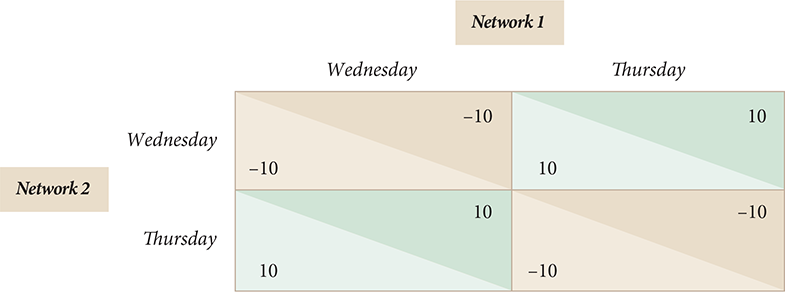
\includegraphics[scale=0.4]{../images/game_theory/networks.png}
	\end{figure}
}

\frame{
	\frametitle{Types of Nash Equilibria}
	\begin{itemize}
	\item Neither network has a dominant strategy; for each, the best choice depends on the choice of its rival.
		\begin{itemize}
		\item If Network 1 opts for Wednesday, then Network 2 prefers Thursday.
		\item If Network 1 chooses Thursday, then Network 2 opts for Wednesday.
		\end{itemize}
	\item[]
	\item In this case there are two Nash Equilibria in pure strategies; each as a different network broadcast on a different day.
	\item[]
	\item Prediction: networks would schedule shows on different nights.
	\item[]
	\item But, we lack a basis for predicting which night each network would choose.
	\end{itemize}
}

\frame{
	\frametitle{Types of Nash Equilibria}
	\begin{itemize}
	\item In our example, the two Networks could potentially exploit \underline{cheap talk} to try and resolve the coordination problem.
	\end{itemize}
	\begin{definition}[Cheap Talk]
	Cheap talk is ``pre-play'' communication where parties communicate without affecting payoffs from the game.
	\end{definition}
	\begin{itemize}
	\item Eg. Network 1 might announce it will broadcast on Wednesday, so Network 2 chooses Thursday.
	\item This type of communication works if there is a clear incentive to be truthful (i.e. higher profits from coordination).
	\end{itemize}
}

\frame{
	\frametitle{Types of Nash Equilibria}
	\begin{itemize}
	\item If cheap talk is not allowed or not credible, then we need a different means to distinguish between potential outcomes.
	\item[]
	\item One possibility arises if there is a solution that has a higher payoff for all parties.
		\begin{itemize}
		\item In this case, we can expect that each player will select that solution even in the absence of any pre-play communication.
		\item This is known as the Pareto Criterion.
		\end{itemize}
	\item[]
	\item As an example, suppose that in Network 1 plays its show on Wednesday, and Network 2 plays its show on Thursday, each firm earns \$15 million.
	\end{itemize}
}

\frame{
	\frametitle{Example: Coordination Between Networks}
	\begin{figure}
	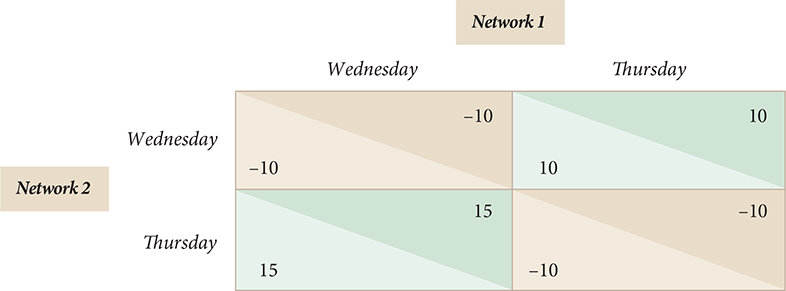
\includegraphics[scale=0.4]{../images/game_theory/networks2.png}
	\end{figure}
}

\frame{
	\frametitle{Types of Nash Equilibria}
	\begin{itemize}
	\item So far, we have assumed that each player uses a \underline{pure strategy}.
	\end{itemize}
	\begin{definition}[Pure Strategy]
	A pure strategy is an action that a player takes in every possible situation in a game.
	\end{definition}
	\begin{itemize}
	\item A pure strategy is a rule telling the player, with certainty, what action to take at each decision point in a game.
	\end{itemize}
}	

\frame{
	\frametitle{Types of Nash Equilibria}
	\begin{itemize}
	\item Players can also use a \underline{mixed strategy}.
	\end{itemize}
	\begin{definition}[Mixed Strategy]
	In a mixed strategy, the player chooses amongst pure strategies according to a probabilities that the player sets.
	\end{definition}
	\begin{itemize}
	\item A mixed strategy is a rule telling the player which method to use to randomly choose amongst possible pure strategies.
	\end{itemize}
}

\frame{
	\frametitle{Contract Example}
	\begin{itemize}
	\item Example: Competition for a contract.
	\item[]
	\item Suppose two design firms, \textit{Upstart} and \textit{Established}, compete for an architectural contract and simultaneously decide if their proposed designs are traditional or modern.
	\end{itemize}
}	

\frame{
	\frametitle{Contract Example}
	\begin{figure}
	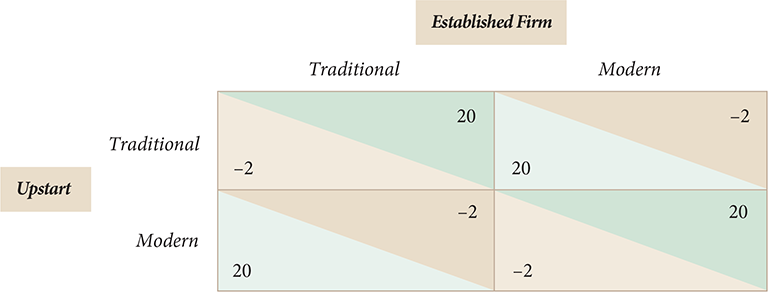
\includegraphics[scale=0.4]{../images/game_theory/design.png}
	\end{figure}
}

\frame{
	\frametitle{Contract Example}
	\begin{itemize}
	\item There is no Nash Equilibrium in pure strategies in this case:
		\begin{itemize}
		\item Upstart's best response to Established is:
			\begin{itemize}
			\item Modern design if Established chooses Traditional.
			\item Traditional design if Established chooses Modern.
			\end{itemize}
		\item[]
		\item Established's best response to Upstart is:
			\begin{itemize}
			\item Modern design if Upstart chooses Modern.
			\item Traditional design if Upstart chooses Traditional.
			\end{itemize}
		\end{itemize}
	\end{itemize}
}

\frame{
	\frametitle{Contract Example}
	\begin{itemize}
	\item There is a Nash Equilibrium in mixed strategies.
	\item[]
	\item Each firm randomizes such that the other is indifferent between the two outcomes.
		\begin{itemize}
		\item Let $\theta$ denote the probability that Established chooses the traditional style.
		\item Upstart's expected payoff is then $[\theta \times (-2)] + [(1-\theta) \times 20] = 20 - 22 \times \theta$ if it picks the traditional style, and $[\theta \times 20] + [(1-\theta) \times (-2)] = -2 +22 \times \theta$ if it picks the modern style.
		\item Upstart will only be indifferent between these two pure strategies if the expected payoffs are equal: $20 -22\theta = -2 +22 \theta$, or $22 - 44 \theta$, or $\theta = 1/2$.
		\item Hence, Established randomizes between the two outcomes with a probability of 1/2. Similarly, Upstart randomizes between the two outcomes with a probability of 1/2.
		\item Nash equilibrium: Each firm chooses the traditional style with a probability of 1/2.
		\end{itemize}
	\end{itemize}
}

\frame{
	\frametitle{Types of Nash Equilibria}
	\begin{itemize}
	\item Both pure and mixed-strategy equilibria can arise in the same game.
	\item[]
	\item Example: Suppose two firms are considering opening gas stations at the same location, but only one station could operate profitably due to small demand. If both firms enter, they both lose \$200k.
	\end{itemize}
}

\frame{
	\frametitle{Entry Game}
	\begin{figure}
	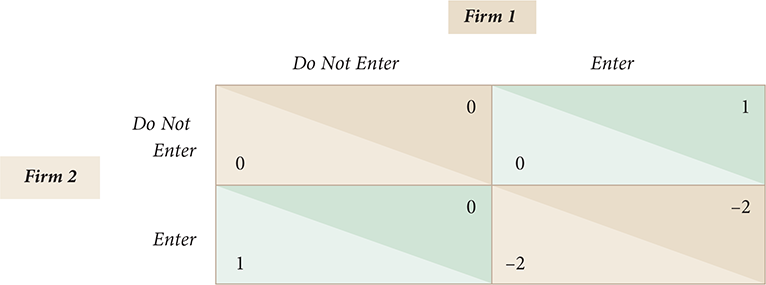
\includegraphics[scale=0.4]{../images/game_theory/entry_static.png}
	\end{figure}
}

\frame{
	\frametitle{Entry Game}
	\begin{itemize}
	\item In this case, neither firm has a dominant strategy. Each firm's best action depends on what the other firm does.
	\item[]
	\item There are three Nash equilibria in total:
		\begin{itemize}
		\item Two Nash equilibria in pure strategies:
			\begin{itemize}
			\item Firm 1 enters and Firm 2 does not.
			\item Firm 2 enters and Firm 1 does not.
			\item Note: players do not know which outcome will arise; cheap talk/Pareto criterion offer no help in this case.
			\end{itemize}
		\item One Nash equilibrium in mixed strategies:
			\begin{itemize}
			\item Each firm enters with a probability of 1/3.
			\item No firm could increase its expected profit by changing its mixed strategy.
			\end{itemize}
		\end{itemize}
	\end{itemize}
}

\section{Information and Rationality}

\frame{
	\frametitle{Outline}
	\begin{enumerate}
	\item Oligopoly Games
	\item[]
	\item Nash Equilibrium
	\item[]
	\item \alert{Information and Rationality}
	\item[]
	\item Using Game Theory to Make Business Decisions
	\item[]
	\item Bargaining
	\item[]
	\item Auctions
	\end{enumerate}
}


\frame{
	\frametitle{Information and Rationality}
	\begin{itemize}
	\item So far, we have assumed players have \underline{complete information}.
		\begin{itemize}
		\item Players know all strategies and associated payoffs (profits).
		\end{itemize}
	\item[]
	\item In more complex settings, players may have \underline{incomplete information}.
		\begin{itemize}
		\item May occur because of \underline{private information} or \underline{high transaction costs}.
		\end{itemize}
	\item[]
	\item We have also assumed players act \underline{rationally}.
		\begin{itemize}
		\item Players use all available information to determine their best strategies.
		\end{itemize}
	\item[]
	\item However, players may have limited powers of calculation, or be unable to determine their best strategies (\underline{bounded rationality}).
	\item[]
	\item When players have incomplete information or exhibit bounded rationality, the Nash equilibrium will be different from games with full information and rationality.
	\end{itemize}
}

\frame{
	\frametitle{Information and Rationality}
	\begin{itemize}
	\item Example: Investment Game
		\begin{itemize}
		\item Google and Samsung decide `to invest' or `do not invest' in complementary products (Chrome OS and Chromebook, respectively).
		\item[]
		\item There is a profit asymmetry from investment:
			\begin{itemize}
			\item A Chromebook with no Chrome OS is worthless.
			\item Chrome OS has value even without the Chromebook.
			\end{itemize}
		\item[]
		\item To start, suppose both firms have full information.
		\end{itemize}
	\end{itemize}
}

\frame{
	\frametitle{Investment Game}
	\begin{figure}
	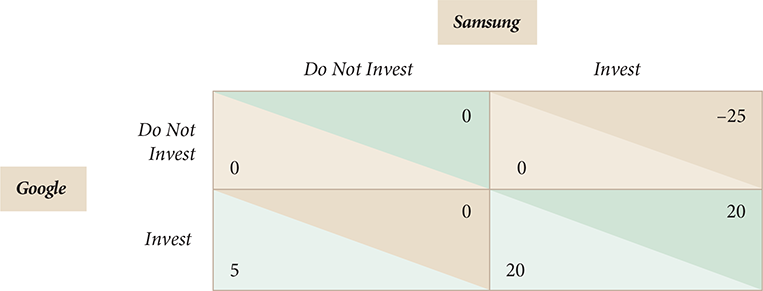
\includegraphics[scale=0.4]{../images/game_theory/invest.png}
	\end{figure}
}

\frame{
	\frametitle{Investment Game}
	\begin{itemize}
	\item If each firm has full information, the unique Nash equilibrium is both firms investing.
		\begin{itemize}
		\item Google's dominant strategy is `invest'.
		\item Samsung's best response is `invest'.
		\end{itemize}
	\item[]
	\item Now suppose that the payoffs (the profits from investing) are not common knowledge.
	\end{itemize}
}

\frame{
	\frametitle{Investment Game}
	\begin{figure}
	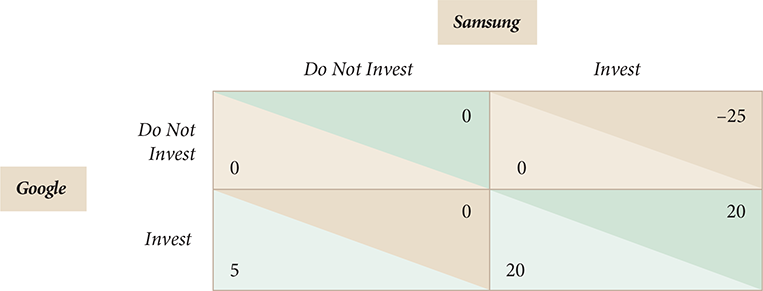
\includegraphics[scale=0.4]{../images/game_theory/invest.png}
	\end{figure}
}

\frame{
	\frametitle{Investment Game}
	\begin{itemize}
	\item With incomplete information, Samsung does not know Google's dominant strategy is to always `invest'.
	\item[]
	\item Given its limited information, Samsung weighs a modest gain vs. a big loss. If it thinks Google will not invest, then Samsung does not invest.
	\item[]
	\item Likely outcome: Samsung and Google fail to coordinate their strategies.
	\item[]
	\item How could Google and Samsung overcome this problem?
	\end{itemize}
}

\frame{
	\frametitle{Information and Rationality}
	\begin{itemize}
	\item We normally assume that rational players consistently choose actions that are in their best interests given the information they have. That is, we assume they are able to choose their profit-maximizing strategies.
	\item[]
	\item However, complexity of strategic interactions may prevent this.
	\item[]
	\item In practice, managers may have limited powers of calculation or logical inference (\underline{bounded rationality}), and may try to maximize profits subject to cognitive limitations.
	\end{itemize}
}

\frame{
	\frametitle{Information and Rationality}
	\begin{itemize}
	\item With bounded rationality, players often resort to \underline{rules of thumb}.
	\item[]
	\item One simple rule of thumb: use a strategy that has worked in the past.
	\item[]
	\item Another common strategy: \underline{maximin}
		\begin{itemize}
		\item This approach maximizes the lowest possible payoff the player might receive.
		\item Goal is to ensure the best possible profit if your rival takes the action that is worst for you.
		\item Example: The maximin solution in the Investment Game is for Google to invest, and for Samsung to not invest.
		\end{itemize}
	\end{itemize}
}

\section{Strategic Decision Making}


\frame{
	\frametitle{Outline}
	\begin{enumerate}
	\item Oligopoly Games
	\item[]
	\item Nash Equilibrium
	\item[]
	\item Information and Rationality
	\item[]
	\item \alert{Using Game Theory to Make Business Decisions}
	\item[]
	\item Bargaining
	\item[]
	\item Auctions
	\end{enumerate}
}


\frame{
	\frametitle{Using Game Theory to Make Business Decisions}
	\begin{itemize}
	\item In reality, many business games are too complex to analyze fully.
	\item[]
	\item However, we can exploit five key insights from game theory to aid in strategic decision making.
		\begin{enumerate}
		\item Dominance
		\item Best response
		\item Point of view
		\item Coordination
		\item Randomize
		\end{enumerate}
	\end{itemize}
}

\frame{
	\frametitle{Using Game Theory to Make Business Decisions}
	\begin{itemize}
	\item[1.] \textit{Dominance}: A manager who has a dominant strategy -- a strategy that is always best no matter what rivals do -- should use it.
	\item[]
	\item[2.] \textit{Best Response}: A manager who does not have a dominant strategy should determine the best responses to the strategies that rivals might use.
	\item[]
	\item[3.] \textit{Point of View}: A manager should consider possible strategies from a rival's vantage point, try to predict which strategy the rival will choose, and select the best response to that strategy.
	\end{itemize}
}

\frame{
	\frametitle{Using Game Theory to Make Business Decisions}
	\begin{itemize}
	\item[4.] \textit{Coordination}: When doing so increases profit, a manager should coordinate with other firms through pre-play communication (cheap talk) or by using legal contracts.
	\item[]
	\item[5.] \textit{Randomize}: A manager may be able to earn a higher profit by keeping rivals guessing using a mixed strategy.
	\end{itemize}
}

\frame{
	\frametitle{Outline}
	\begin{enumerate}
	\item Oligopoly Games
	\item[]
	\item Nash Equilibrium
	\item[]
	\item Information and Rationality
	\item[]
	\item Using Game Theory to Make Business Decisions
	\item[]
	\item \alert{Bargaining}
	\item[]
	\item Auctions
	\end{enumerate}
}


\frame{
	\frametitle{Bargaining}
	\begin{itemize}
	\item Bargaining is common in many business situations.
		\begin{itemize}
		\item Managers and employees bargain over working conditions.
		\item Firms may bargain with suppliers or distributors.
		\end{itemize}
	\item[]
	\item Game theory can be used to understand bargaining situations.
		\begin{itemize}
		\item \underline{Bargaining game}: Any situation in which two or more parties with different interests or objectives negotiate voluntarily over the terms of some interaction, such as the transfer of a good from one party to another.
		\item[]
		\item Solution to game: Nash Bargaining solution.
			\begin{itemize}
			\item Note: Nash Bargaining solution $\neq$ Nash equilibrium.
			\end{itemize}
		\end{itemize}
	\end{itemize}
}

\frame{
	\frametitle{Bargaining}
	\begin{itemize}
	\item A bargaining game is a \textit{cooperative} game.
		\begin{itemize}
		\item Parties are trying to decide how to divide profits or some other payoff.
		\end{itemize}
	\item[]
	\item Nash bargaining solution determines \textit{efficient} division of payoff.
		\begin{itemize}
		\item No alternative outcome that would be better for both parties or strictly better for one party and no worse for the other.
		\end{itemize}
	\item[]
	\item As an example, let's revisit the interaction between American and United.
		\begin{itemize}
		\item But now, we will assume US antitrust laws have changed such that the firms can bargain over output levels and reach a binding agreement.
		\end{itemize}
	\end{itemize}
}

\frame{
	\frametitle{Bargaining}
	\begin{figure}
	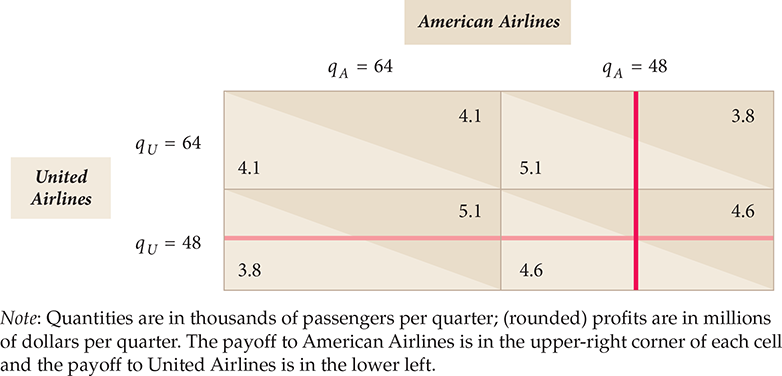
\includegraphics[scale=0.4]{../images/game_theory/au1.png}
	\end{figure}
}

\frame{
	\frametitle{Bargaining}
	\begin{itemize}
	\item With Nash Bargaining, the division of payoffs depends on the outside option available to each party.
		\begin{itemize}
		\item The value of the outside option is the \underline{disagreement} point; it is the outcome that arises if no agreement is reached (call this $d$).
			\begin{itemize}
			\item If United and American cannot reach an agreement they revert to the non-cooperative outcome: $d_{A} = d_{U} = 4.1$.
			\end{itemize}
		\item If an agreement is reached, each party receives a payoff of $\pi$, and a \underline{net surplus} of $\pi - d$.
		\end{itemize}
	\item[]
	\item The Nash Bargaining solution maximizes the product of the net surplus for the two firms:
		\begin{align*}
		NP = [\pi_{A} - d_{A}] \times [\pi_U - d_U]
		\end{align*}
	\end{itemize}
}

\frame{
	\frametitle{Bargaining}
	\begin{itemize}
	\item There are four possible outcomes for a bargain between United and American:
		\begin{enumerate}
		\item Both produce 64k: $NP=0$.
		\item American 64k, United 48k: $NP<0$.
		\item American 64k, United 48k: $NP<0$.
		\item Both produce 48k: $NP=[4.6-4.1]\times[4.6-4.1]=0.25$.
		\end{enumerate}
	\item[]
	\item Nash bargaining predicts both American and United would fly 48 thousand passengers.
	\end{itemize}
}

\frame{
	\frametitle{Bargaining}
	\begin{itemize}
	\item If United and American could bargain about how they set their output levels in an oligopoly game, they could reach an efficient outcome that maximizes the Nash product.
	\item[]
	\item Such an agreement creates a cartel and raises the firms' profits.
		\begin{itemize}
		\item Gain for firms is more than offset by loss in consumer surplus.
		\item Consequently, such agreements are illegal in most developed countries under antitrust and competition laws.
		\end{itemize}
	\end{itemize}
}

\frame{
	\frametitle{Bargaining}
	\begin{itemize}
	\item The Nash Bargaining solution presumes that the parties achieve an efficient outcome where neither party could be made better off without harming the other party.
	\item[]
	\item However, in the real world, bargaining often yields inefficient outcomes.
		\begin{itemize}
		\item The bargaining process is often time consuming, which delays the start of the benefit flow, and therefore reduces the value of benefits overall.
			\begin{itemize}
			\item This is common with strikes.
			\end{itemize}
		\item Bounded rationality and incomplete information also matter; parties do their best, but are unable to determine the best possible strategies, leading to mistakes that are costly for both parties.
		\end{itemize}
	\end{itemize}
}


\frame{
	\frametitle{Outline}
	\begin{enumerate}
	\item Oligopoly Games
	\item[]
	\item Nash Equilibrium
	\item[]
	\item Information and Rationality
	\item[]
	\item Using Game Theory to Make Business Decisions
	\item[]
	\item Bargaining
	\item[]
	\item \alert{Auctions}
	\end{enumerate}
}


\frame{
	\frametitle{Auctions}
	\begin{definition}[Auction]
	A sale in which a good or service is sold to the highest bidder.
	\end{definition}
	\begin{itemize}
	\item Game theory can be used to understand behaviour in auctions.
		\begin{itemize}
		\item An auction is a game in which players (called \underline{bidders}) devise bidding strategies without knowing the payoff functions of other players.
		\item Bidders need to know the rules of the game:
			\begin{itemize}
			\item The number of units being sold.
			\item The format of bidding.
			\item The value that potential bidders place on the good.
			\end{itemize}
		\end{itemize}
	\end{itemize}
}

\frame{
	\frametitle{Auctions}
	\begin{itemize}
	\item Auctions are frequently used in practice:
		\begin{itemize}
		\item Government auctions:
			\begin{itemize}
			\item Government procurement, auctions for electricity and transport markets, auctions to concede portions of the airwaves for radio stations, mobile phones and wireless internet access; auctions for oil and gas leases.
			\end{itemize}
		\item[]
		\item Market transactions:
			\begin{itemize}
			\item Goods commonly sold at auction are natural resource such as timber and drilling rights for oil, as well as houses, cars, agricultural products, horses, antiques and art. And of course, goods online in sites like eBay.
			\end{itemize}
		\end{itemize}
	\end{itemize}
}

\frame{
	\frametitle{Elements of Auctions}
	\begin{itemize}
		\item Number of units: auctions can be used to sell one or many units of a good.
		\item Format of bidding:
			\begin{itemize}
			\item  \underline{English auction}: Ascending-bid auction process where the good is sold to the last bidder for the highest bid. Commonly used to sell art/antiques.
			\item \underline{Dutch auction}: Descending-bid auction process where the seller reduces the price until someone accepts it and buys at that price. Often used in government procurement.
			\item \underline{Sealed-bid auction}: Bidders submit bids simultaneously without seeing anyone else's bid and highest bidder wins. In a 1st price sealed-bid auction, the winner pays its own, highest bid. In a 2nd price sealed-bid auction, the winner pays the amount bid by the 2nd highest bidder.
			\end{itemize}
		\item Value:
			\begin{itemize}
			\item \underline{Private value}: Individual bidders know how much the good is worth to them, but not how much other bidders value it.
			\item \underline{Common value}: The good has the same value to everyone, but no bidder knows exactly what that value is.
			\end{itemize}
		\end{itemize}
}

\frame{
	\frametitle{Second Price Sealed Bid Auctions}
	\begin{itemize}
	\item Rules:
		\begin{itemize}
		\item Each bidder has a different private value for a single indivisible good.
		\item Bidders simultaneously submit sealed bids without knowledge of other bids.
		\end{itemize}
	\item Design of auction means that amount that you bid affects whether you win, but it does not affect how much you pay if you win (which is equal to the second-highest bid).
	\item Best strategy: Bid your highest value.
		\begin{itemize}
		\item This strategy weakly dominates all others.
		\item Ex: Suppose that you value a folk art carving at \$100. If you bid \$100 and win, your $CS=100 - \text{2nd price}$. If you bid less than \$100, you risk not winning. If you bid more than \$100, you risk ending up with negative $CS$.
		\item Thus, bidding \$100 leaves you \textit{at least as well off} as bidding any other value.
		\end{itemize}
	\end{itemize}
}

\frame{
	\frametitle{English Auctions}
	\begin{itemize}
	\item Rules:
		\begin{itemize}
		\item Each bidder has a different private value for a single indivisible good.
		\item Ascending-bid auction process where the good is sold to the last bidder for the highest bid.
		\end{itemize}
	\item Design of auction means that amount you bid affects whether you win and how much you pay.
	\item Best strategy: Raise the current highest bid as long as that value is less than the value you place on the good.
		\begin{itemize}
		\item Ex: Again suppose that you value a folk art carving at \$100. If you bid an amount $b$ and win, $CS =100- b$. $CS$ is positive or zero for $b\leq100$, but negative if $b>100$. So it is best to raise bids up to \$100 and stop there.
		\item If all participants bid up to their value, the winner will pay slightly more than the value of the second-highest bidder. Thus, the outcome of an English auction is essentially the same is a in a sealed-bid, second-price auction.
		\end{itemize}
	\end{itemize}
}

\frame{
	\frametitle{Other Auctions}
	\begin{itemize}
	\item Two other common private value auctions:
		\begin{itemize}
		\item Dutch Auction: Descending-bid auction where the seller reduces the price until someone accepts the offered price and buys at that price.
		\item First-Price Sealed-Bid Auction: Bidders submit bids simultaneously without seeing other bids. Highest bidder wins and pays amount of bid.
		\end{itemize}
	\item In both cases, the amount that you bid affects whether you win and pay.
	\item The best strategy in both auctions is to bid an amount that is equal to, or slightly greater than what you expect will be the second-highest bid, given that your value is the highest.
		\begin{itemize}
		\item Bidders shade bids to less than their value to balance the effect of decreasing the probability of winning and increasing $CS$. Bid depends on beliefs about strategies of rivals.
		\end{itemize}
	\end{itemize}
}

\frame{
	\frametitle{Auctions}
	\begin{itemize}
	\item Key point: Expected outcome is the same across private value auctions.
		\begin{itemize}
		\item Winner is the person with the highest value, and the winner pays roughly the second-highest value.
		\end{itemize}
	\item[]
	\item Is there any reason that a seller still might choose one format over an alternative?
	\end{itemize}
}

\frame{
	\frametitle{Auctions}
	\begin{itemize}
	\item Key feature of \underline{common-value} auctions: the Winner's Curse.
		\begin{itemize}
		\item Winner's bid exceeds the value of item up for bid; winner pays too much.
		\item Occurs due to uncertainty about the true value of the good.
			\begin{itemize}
			\item E.g. Timber land auctions/auctions for oil and gas leases.
			\end{itemize}
		\end{itemize}
	\item Best strategy to avoid Winner's Curse: Shade/reduce bids to below estimates of value.
		\begin{itemize}
		\item The amount of reduction depends on number of other bidders; more bidders $\implies$ more likely winning bid is an overestimate.
		\end{itemize}
	\item While Winner's Curse is a well known phenomenon, there is strong empirical evidence it continues to happen in practice (e.g in the corporate acquisition market).
		\begin{itemize}
		\item One possible explanation: Bounded rationality.
		\end{itemize}
	\end{itemize}
}

\frame{
	\frametitle{Takeaways}
	\begin{enumerate}
	\item Insights from game theory can be used to improve outcomes when making strategic decisions.
	\item[]
	\item Bargaining can lead to efficient outcomes.
	\item[]
	\item Best strategy in most auctions is to bid your valuation, but it may be useful to shade bids to avoid the Winner's Curse.
	\end{enumerate}
}

\end{document}

